\section{Einführung}
Ziel der OOA (Analyse) ist es, die Wünsche und Anforderungen des Auftraggebers zu erfassen und beschreiben. OOA ist technologie unabhängig und entählt keine Optimierungen. Objektorientierung hilft dabei, komplexe System mit angemessenen Mitteln zu dokumentieren, da diese Konzept gut auf die Reelle Welt überführt werden kann. Zur Visualisierung wird oft eine Programmiersprachen-unabhängiges Diagram 'UML' (Unified Modeling Language) verwendet.\\
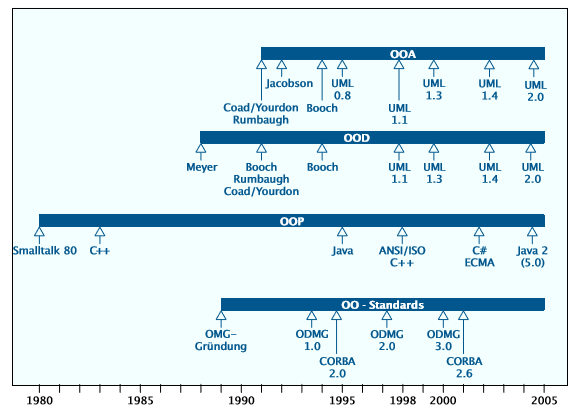
\includegraphics[width=\columnwidth]{Images/geschichte}


OOD (Design) ist die Vorstufe der Implementierung und verfeinert die OOA mit Deteils. Die Architektur zusammen Optimierungen und Technologien werden hier festgelegt.

\textbf{tl:dr} OOA sagt \textit{was} das System können muss, OOD sagt \textit{wie} das System das das macht. 